\documentclass{article}
\usepackage{booktabs}
\usepackage[margin=1in]{geometry}
\usepackage{caption}
\usepackage{graphicx}

\begin{document}
	
	\section*{Models}
	
	\begin{table}[h!]
		\centering
		\caption*{Models' architecture}
		\begin{tabular}{@{}lccccc@{}}
			\midrule[0.2pt]
			& \textbf{Enc. Blocks} & \textbf{Dec. Blocks} & \textbf{Pos. Encoding} & \textbf{Embedding} & \textbf{Output Steps} \\
			\midrule[0.2pt]
			\textbf{Model 1} & 1 & 1 & Learnable & 8 & 4 \\
			\addlinespace[16pt]
		\end{tabular}
	\end{table}
	
	\begin{table}[h!]
		\centering
		\caption*{\textbf{Model 1} Results}
		\begin{tabular}{@{}lccccc@{}}
			\multicolumn{6}{c}{\textbf{Yearly}} \\
			\midrule[0.2pt]
				& \textbf{Finance} & \textbf{Macro} & \textbf{Micro} & \textbf{Industry} & \textbf{Demographic} \\
			\midrule[0.2pt]
			Train Loss & ? & ? & ? & ? & ? \\
			Test Loss  & ? & ? & ? & ? & ? \\[4pt]
			ID         & ? & ? & ? & ? & ? \\
			\addlinespace[16pt]
			
			\multicolumn{6}{c}{\textbf{Quarterly}} \\
			\midrule[1pt]
			& \textbf{Finance} & \textbf{Macro} & \textbf{Micro} & \textbf{Industry} & \textbf{Demographic} \\
			\midrule[0.2pt]
			Train Loss & 0.4248 & 0.1124 & 0.6787 & 0.7141 & 0.1186 \\
			Test Loss  & 0.1458 & 0.1177 & 0.1321 & 0.1772 & 0.1419 \\[4pt]
			ID         & 1321 & 1041 & 840 & 873 & 1345 \\
		\end{tabular}
	\end{table}
	
	\begin{figure}[htbp]
		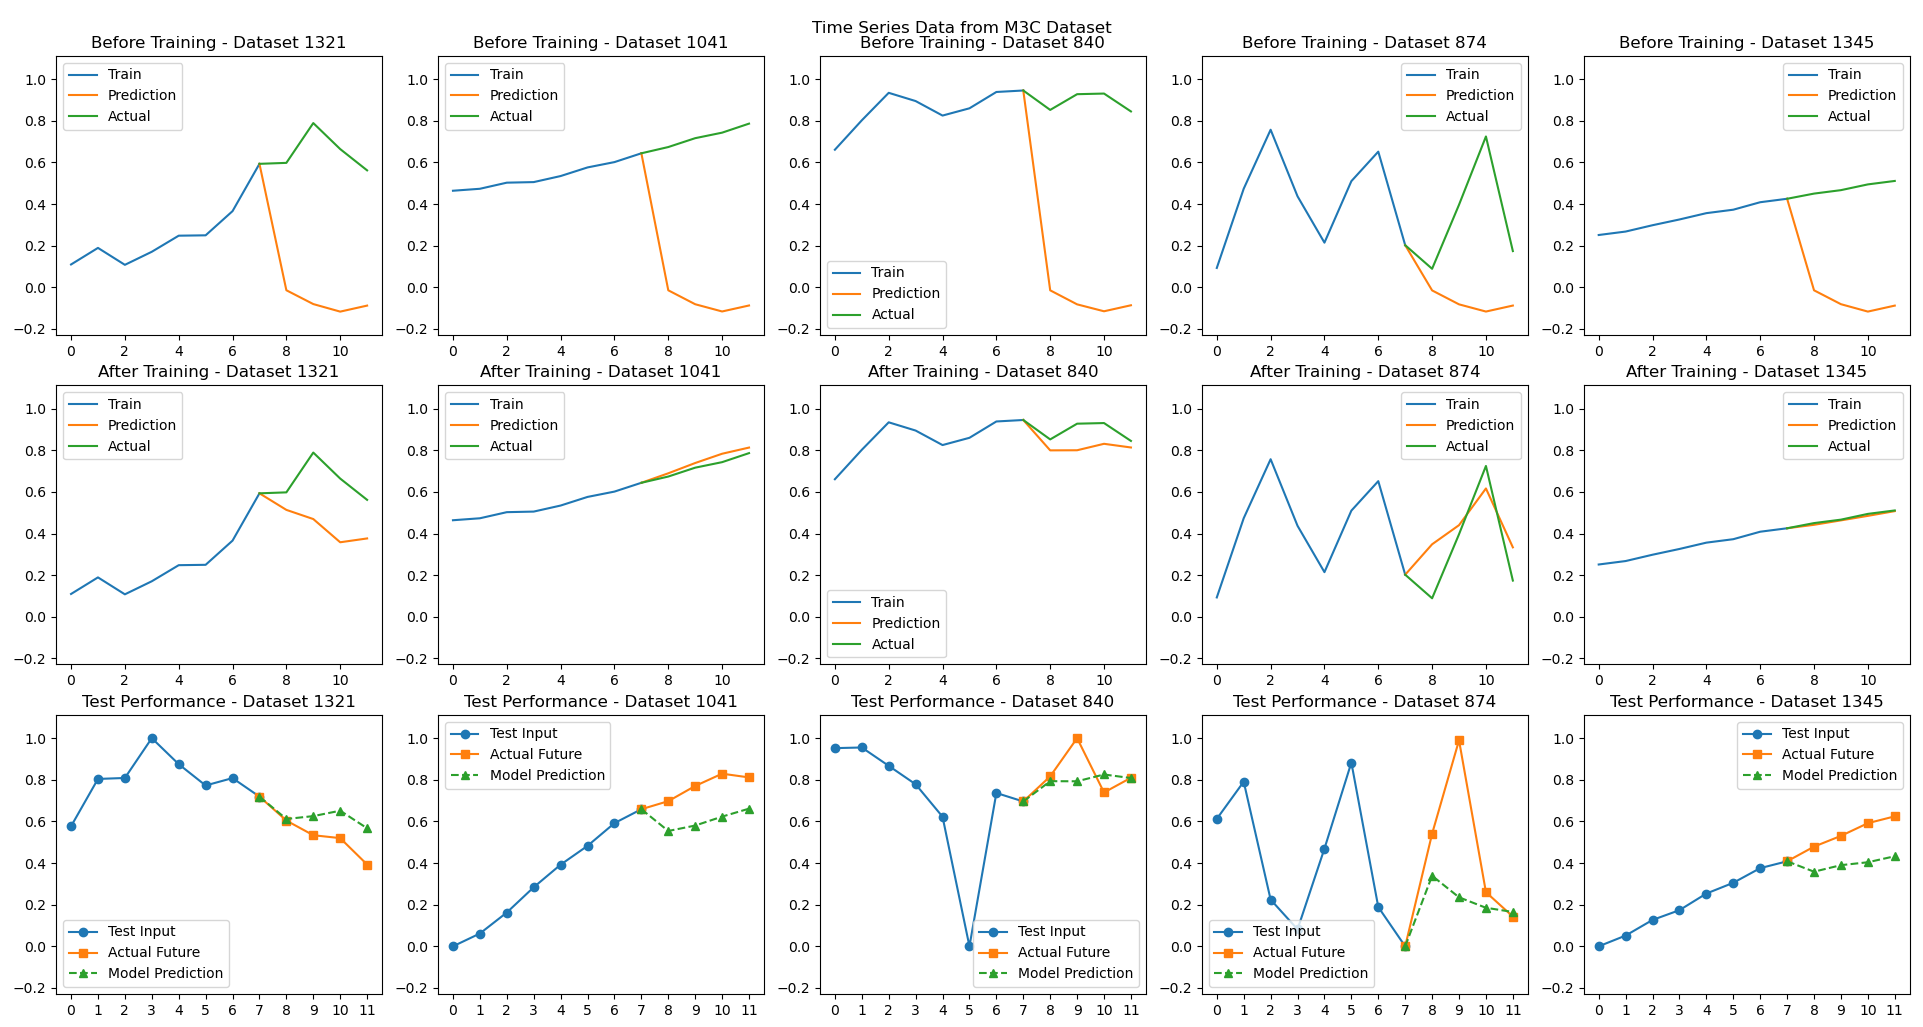
\includegraphics[width=520pt]{model1.png}
	\end{figure}
	
\end{document}
